% !Tex root = main.tex
%-----------------------------------------------------------------------------------------------------------------------------------------------%
%	The MIT License (MIT)
%
%	Copyright (c) 2019 Jan Küster
%
%	Permission is hereby granted, free of charge, to any person obtaining a copy
%	of this software and associated documentation files (the "Software"), to deal
%	in the Software without restriction, including without limitation the rights
%	to use, copy, modify, merge, publish, distribute, sublicense, and/or sell
%	copies of the Software, and to permit persons to whom the Software is
%	furnished to do so, subject to the following conditions:
%	
%	THE SOFTWARE IS PROVIDED "AS IS", WITHOUT WARRANTY OF ANY KIND, EXPRESS OR
%	IMPLIED, INCLUDING BUT NOT LIMITED TO THE WARRANTIES OF MERCHANTABILITY,
%	FITNESS FOR A PARTICULAR PURPOSE AND NONINFRINGEMENT. IN NO EVENT SHALL THE
%	AUTHORS OR COPYRIGHT HOLDERS BE LIABLE FOR ANY CLAIM, DAMAGES OR OTHER
%	LIABILITY, WHETHER IN AN ACTION OF CONTRACT, TORT OR OTHERWISE, ARISING FROM,
%	OUT OF OR IN CONNECTION WITH THE SOFTWARE OR THE USE OR OTHER DEALINGS IN
%	THE SOFTWARE.
%	
%
%-----------------------------------------------------------------------------------------------------------------------------------------------%


%============================================================================%
%
%	DOCUMENT DEFINITION
%
%============================================================================%

%we use article class because we want to fully customize the page and don't use a cv template
\documentclass[10pt,A4]{article}	


%----------------------------------------------------------------------------------------
%	ENCODING
%----------------------------------------------------------------------------------------

% we use utf8 since we want to build from any machine
\usepackage[utf8]{inputenc}		

%----------------------------------------------------------------------------------------
%	LOGIC
%----------------------------------------------------------------------------------------

% provides \isempty test
\usepackage{xstring, xifthen}

%----------------------------------------------------------------------------------------
%	FONT BASICS
%----------------------------------------------------------------------------------------

% some tex-live fonts - choose your own

%\usepackage[defaultsans]{droidsans}
%\usepackage[default]{comfortaa}
%\usepackage{cmbright}
\usepackage[default]{raleway}
%\usepackage{fetamont}
%\usepackage[default]{gillius}
%\usepackage[light,math]{iwona}
%\usepackage[thin]{roboto} 

% set font default
\renewcommand*\familydefault{\sfdefault} 	
\usepackage[T1]{fontenc}

% more font size definitions
\usepackage{moresize}

%----------------------------------------------------------------------------------------
%	FONT AWESOME ICONS
%---------------------------------------------------------------------------------------- 

% include the fontawesome icon set
\usepackage{fontawesome}

% use to vertically center content
% credits to: http://tex.stackexchange.com/questions/7219/how-to-vertically-center-two-images-next-to-each-other
\newcommand{\vcenteredinclude}[1]{\begingroup
\setbox0=\hbox{\includegraphics{#1}}%
\parbox{\wd0}{\box0}\endgroup}

% use to vertically center content
% credits to: http://tex.stackexchange.com/questions/7219/how-to-vertically-center-two-images-next-to-each-other
\newcommand*{\vcenteredhbox}[1]{\begingroup
\setbox0=\hbox{#1}\parbox{\wd0}{\box0}\endgroup}

% icon shortcut
\newcommand{\icon}[3] { 							
	\makebox(#2, #2){\textcolor{maincol}{\csname fa#1\endcsname}}
}	

% icon with text shortcut
\newcommand{\icontext}[4]{ 						
	\vcenteredhbox{\icon{#1}{#2}{#3}}  \hspace{2pt}  \parbox{0.9\mpwidth}{\textcolor{#4}{#3}}
}

% icon with website url
\newcommand{\iconhref}[5]{ 						
    \vcenteredhbox{\icon{#1}{#2}{#5}}  \hspace{2pt} \href{#4}{\textcolor{#5}{#3}}
}

% icon with email link
\newcommand{\iconemail}[5]{ 						
    \vcenteredhbox{\icon{#1}{#2}{#5}}  \hspace{2pt} \href{mailto:#4}{\textcolor{#5}{#3}}
}

%----------------------------------------------------------------------------------------
%	PAGE LAYOUT  DEFINITIONS
%----------------------------------------------------------------------------------------

% page outer frames (debug-only)
% \usepackage{showframe}		
%package to display URLs as such in the pdf
%\usepackage{hyperref}

% we use paracol to display breakable two columns
\usepackage{paracol}

% define page styles using geometry
\usepackage[a4paper]{geometry}

% remove all possible margins
\geometry{top=1cm, bottom=1cm, left=1cm, right=1cm}

\usepackage{fancyhdr}
\pagestyle{empty}

% space between header and content
% \setlength{\headheight}{0pt}

% indentation is zero
\setlength{\parindent}{0mm}

%----------------------------------------------------------------------------------------
%	TABLE /ARRAY DEFINITIONS
%---------------------------------------------------------------------------------------- 

% extended aligning of tabular cells
\usepackage{array}

% custom column right-align with fixed width
% use like p{size} but via x{size}
\newcolumntype{x}[1]{%
>{\raggedleft\hspace{0pt}}p{#1}}%


%----------------------------------------------------------------------------------------
%	GRAPHICS DEFINITIONS
%---------------------------------------------------------------------------------------- 

%for header image
\usepackage{graphicx}

% use this for floating figures
% \usepackage{wrapfig}
% \usepackage{float}
% \floatstyle{boxed} 
% \restylefloat{figure}

%for drawing graphics		
\usepackage{tikz}				
\usetikzlibrary{shapes, backgrounds,mindmap, trees}

%----------------------------------------------------------------------------------------
%	Color DEFINITIONS
%---------------------------------------------------------------------------------------- 
\usepackage{transparent}
\usepackage{color}

% primary color
\definecolor{maincol}{RGB}{ 225, 0, 0 }

% accent color, secondary
% \definecolor{accentcol}{RGB}{ 250, 150, 10 }

% dark color
\definecolor{darkcol}{RGB}{ 70, 70, 70 }

% light color
\definecolor{lightcol}{RGB}{245,245,245}


% Package for links, must be the last package used
\usepackage[hidelinks]{hyperref}

% returns minipage width minus two times \fboxsep
% to keep padding included in width calculations
% can also be used for other boxes / environments
\newcommand{\mpwidth}{\linewidth-\fboxsep-\fboxsep}
	


%============================================================================%
%
%	CV COMMANDS
%
%============================================================================%

%----------------------------------------------------------------------------------------
%	 CV LIST
%----------------------------------------------------------------------------------------

% renders a standard latex list but abstracts away the environment definition (begin/end)
\newcommand{\cvlist}[1] {
	\begin{itemize}{#1}\end{itemize}
}

%----------------------------------------------------------------------------------------
%	 CV TEXT
%----------------------------------------------------------------------------------------

% base class to wrap any text based stuff here. Renders like a paragraph.
% Allows complex commands to be passed, too.
% param 1: *any
\newcommand{\cvtext}[1] {
	\begin{tabular*}{1\mpwidth}{p{0.98\mpwidth}}
		\parbox{1\mpwidth}{#1}
	\end{tabular*}
}

%----------------------------------------------------------------------------------------
%	CV SECTION
%----------------------------------------------------------------------------------------

% Renders a a CV section headline with a nice underline in main color.
% param 1: section title
\newcommand{\cvsection}[1] {
	\vspace{14pt}
	\cvtext{
		\textbf{\LARGE{\textcolor{darkcol}{\uppercase{#1}}}}\\[-4pt]
		\textcolor{maincol}{ \rule{0.1\textwidth}{2pt} } \\
	}
}

%----------------------------------------------------------------------------------------
%	META SKILL
%----------------------------------------------------------------------------------------

% Renders a progress-bar to indicate a certain skill in percent.
% param 1: name of the skill / tech / etc.
% param 2: level (for example in years)
% param 3: percent, values range from 0 to 1
\newcommand{\cvskill}[3] {
	\begin{tabular*}{1\mpwidth}{p{0.72\mpwidth}  r}
 		\textcolor{black}{\textbf{#1}} & \textcolor{maincol}{#2}\\
	\end{tabular*}%
	
	\hspace{4pt}
	\begin{tikzpicture}[scale=1,rounded corners=2pt,very thin]
		\fill [lightcol] (0,0) rectangle (1\mpwidth, 0.15);
		\fill [maincol] (0,0) rectangle (#3\mpwidth, 0.15);
  	\end{tikzpicture}%
}


%----------------------------------------------------------------------------------------
%	 CV EVENT
%----------------------------------------------------------------------------------------

% Renders a table and a paragraph (cvtext) wrapped in a parbox (to ensure minimum content
% is glued together when a pagebreak appears).
% Additional Information can be passed in text or list form (or other environments).
% the work you did
% param 1: time-frame i.e. Sep 14 - Jan 15 etc.
% param 2:	 event name (job position etc.)
% param 3: Customer, Employer, Industry
% param 4: Short description
% param 5: work done (optional)
% param 6: technologies include (optional)
% param 7: achievements (optional)
\newcommand{\cvevent}[7] {
	
	% we wrap this part in a parbox, so title and description are not separated on a pagebreak
	% if you need more control on page breaks, remove the parbox
	\parbox{\mpwidth}{
		\begin{tabular*}{1\mpwidth}{p{0.72\mpwidth}  r}
	 		\textcolor{black}{\textbf{#2}} & \colorbox{maincol}{\makebox[0.25\mpwidth]{\textcolor{white}{#1}}} \\
			\textcolor{maincol}{\textbf{#3}} & \\
		\end{tabular*}\\[8pt]
	
		\ifthenelse{\isempty{#4}}{}{
			\cvtext{#4}\\
		}
	}

	\ifthenelse{\isempty{#5}}{}{
		\vspace{9pt}
		{#5}
	}

	\ifthenelse{\isempty{#6}}{}{
		\vspace{9pt}
		\cvtext{\textbf{Technologies include:}}\\
		{#6}
	}

	\ifthenelse{\isempty{#7}}{}{
		\vspace{9pt}
		\cvtext{\textbf{Achievements include:}}\\
		{#7}
	}
	\vspace{14pt}
}

%----------------------------------------------------------------------------------------
%	 CV META EVENT
%----------------------------------------------------------------------------------------

% Renders a CV event on the sidebar
% param 1: title
% param 2: subtitle (optional)
% param 3: customer, employer, etc,. (optional)
% param 4: info text (optional)
\newcommand{\cvmetaevent}[4] {
	\textcolor{maincol} {\cvtext{\textbf{\begin{flushleft}#1\end{flushleft}}}}

	\ifthenelse{\isempty{#2}}{}{
	\textcolor{darkcol} {\cvtext{\textbf{#2}} }
	}

	\ifthenelse{\isempty{#3}}{}{
		\cvtext{{ \textcolor{darkcol} {#3} }}\\
	}

	\cvtext{#4}\\[14pt]
}

%---------------------------------------------------------------------------------------
%	QR CODE
%----------------------------------------------------------------------------------------

% Renders a qrcode image (centered, relative to the parentwidth)
% param 1: percent width, from 0 to 1
\newcommand{\cvqrcode}[1] {
	\begin{center}
		
\includegraphics[width={#1}\mpwidth]{qrcode}
	\end{center}
}


%============================================================================%
%
%
%
%	DOCUMENT CONTENT
%
%
%
%============================================================================%
\begin{document}
\columnratio{0.31}
\setlength{\columnsep}{2.2em}
\setlength{\columnseprule}{4pt}
\colseprulecolor{lightcol}
\begin{paracol}{2}
\begin{leftcolumn}
%---------------------------------------------------------------------------------------
%	META IMAGE
%----------------------------------------------------------------------------------------
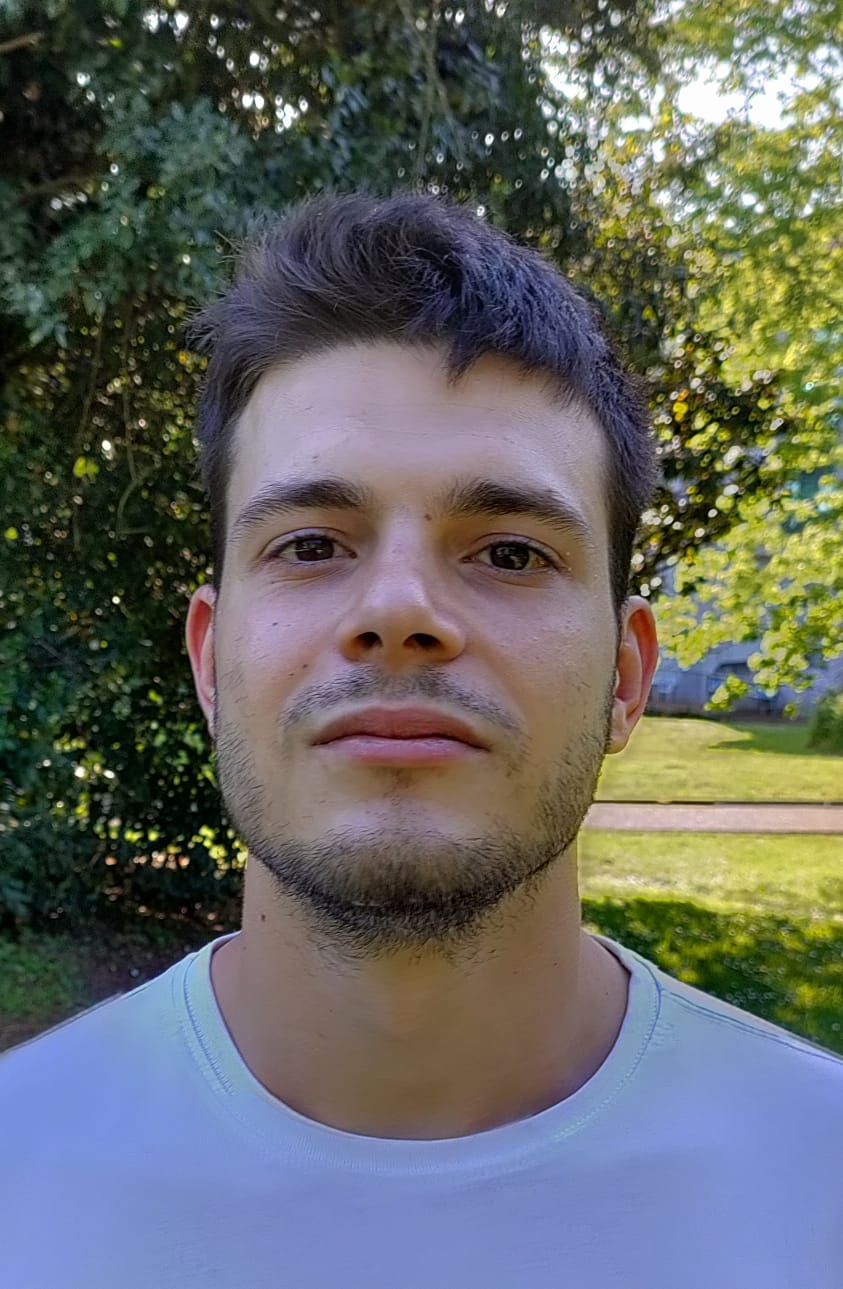
\includegraphics[width=\linewidth]{foto_perfil_buena.jpg}	%trimming relative to image size

%---------------------------------------------------------------------------------------
%	META SKILLS
%----------------------------------------------------------------------------------------
\cvsection{SKILLS}

\cvskill{R} {+2 yrs} {1} \\[-2pt]

\cvskill{LaTeX} {+1 yrs} {0.75}\\ [-2pt]

\cvskill{Python} {-1 yrs} {0.5} \\[-2pt]

\cvskill{SQL} {-1 yrs} {0.5}\\[-2pt]


\vfill\null
\cvsection{CONTACT}
	
\icontext{MapMarker}{12}{Avda. de Lugo 32 2ºA\\15707 Santiago de Compostela, A Coruña}{black}\\[6pt]
\icontext{MobilePhone}{12}{+34 619 56 09 90}{black}\\[6pt]
\iconemail{Envelope}{12}{diegogasn@gmail.com}{diegogasn@gmail.com}{black}\\[6pt]

\vfill\null
\cvqrcode{0.7}

%---------------------------------------------------------------------------------------
%	EDUCATION
%----------------------------------------------------------------------------------------
\newpage
\cvsection{EDUCATION}

\cvmetaevent
{2019 - 2022}
{Interuniversity Master in Statistical Techniques}
{Universidade de Santiago de Compostela - Faculty of Maths}
{Techniques included:
\cvlist{
\item Parametric and non-parametric analysis and inference
\item Optimization
\item Regression
\item Data representation
\item Time series
\item Supervised and unsupervised statistical learning
\item Machine learning
\item Queries and data base management}
Good adaptation to remote learning both before and after the pandemic.\\
Average grade: 7.6222}

\cvmetaevent
{2014 -2019}
{B. Degree in Psychology.}
{Universidade de Santiago de Compostela - Faculty of Psychology}
{Bachelor's thesis about the use of the encephalogram to digitally authenticate individuals. \\
Erasmus + program at the Univerzita Karlova, Prague.\\
Average grade: 8.025}

\vfill\null
\cvqrcode{0.7}

%---------------------------------------------------------------------------------------
%	CERTIFICATION
%----------------------------------------------------------------------------------------
\newpage
\cvsection{CERTIFICATIONS}

\cvmetaevent
{Udemy - Intermediate Python Inmersive Training}
{November, 22}
{}
{}

\cvmetaevent
{Cambridge CAE C1}
{March, 14}
{}
{}

\cvmetaevent
{TOEFL}
{March, 19}
{}
{Score = 100}

\cvmetaevent
{Judo Black Belt}
{November,2018}
{}
{2nd DAN}


\cvmetaevent
{Driving license}
{November, 2014}
{}
{B - class}


\vfill
\cvqrcode{0.7}

\newpage
\mbox{} % hotfix to place qrcode on the bottom when there are not other elements
\vfill
\cvqrcode{0.7}

\end{leftcolumn}
\begin{rightcolumn}
%---------------------------------------------------------------------------------------
%	TITLE  HEADER
%----------------------------------------------------------------------------------------
\fcolorbox{white}{darkcol}{\begin{minipage}[c][3.5cm][c]{1\mpwidth}
	\begin {center}
		\HUGE{ \textbf{ \textcolor{white}{ \uppercase{ DIEGO GARCIA SANCHEZ } } } } \\[-24pt]
		\textcolor{white}{ \rule{0.1\textwidth}{1.25pt} } \\[4pt]
		\large{ \textcolor{white} {Psychologist | Statistical Technician | Data Analyst} }
	\end {center}
\end{minipage}} \\[14pt]
\vspace{-12pt}

%---------------------------------------------------------------------------------------
%	PROFILE
%----------------------------------------------------------------------------------------
\vfill\null
\cvsection{PROFILE}

\cvtext{Graduated as a psychologist, I am focusing on the skills acquired in my Master's degree on statistical techniques. A strong theoretical background promts a specialized profile for analysing psychological-related data. Other fields under my scope include market research, sensory analysis and a genuine interest in bringing the latest technologies to the end user.\\

I stand out for having a good intuition of the human mind and trained critical thinking. I try to keep my knowledge of the world up to date, I score high on intellectual curiosity and openness to experience. Work ethic is a feature commonly highlighted by previous employers too.\\

Highly motivated to work in a team, both in big companies and small teams.\\

From a life dedicated to judo I learned values such as discipline, perseverance and respect.\\
}

%---------------------------------------------------------------------------------------
%	WORK EXPERIENCE
%----------------------------------------------------------------------------------------
\vfill\null
\cvsection{WORK EXPERIENCE}

\cvevent
	{Sept 20 - Now}
	{Co-founder | Head of Data and Evaluation}
	{CóidoME}
	{Project conceived to offer training services in mental health, offering practical and handy solutions to teenagers, promoted by \textit{Xunta de Galicia}. 			The project is currently in an early development phase. My main function is the evaluation of the activities carried out.}
	{\cvlist{
		\item \url{https://coidome.com/}
		\item Questionnary design and analysis
		\item Evaluation of the project and report of results
		\item Occasional speaker in training sessions
		\item Main responsible of compilance with regulations
	}}
	{\cvlist{
		\item R for data analysis
	}}
	{\cvlist {
		\item High average perceived utility among the students
		\item Relevant findings about psychological topics the sample was concerned about
	}}

\vfill\null
\cvevent
	{Oct 22 - Now}
	{Data Analyst | Web Engine Evaluator}
	{Telus International AI}
	{Analysis and evaluation of web engine results.}
	{\cvlist{
		\item Geographical data analysis and evaluation
		\item Image web search analysis and evaluation
		\item Evaluation and analysis of search engine suggestons
	}}
	{\cvlist {
		\item XLM for personal tracking of records
		\item Python for automation of monthly calculations
	}}
	{\cvlist{
		\item Satisfactory integration with the team
		\item Succesfully completed training for the position
	}}

\vfill\null
\cvevent
	{Oct 21 - May 22}
	{English Teacher}
	{Piccadilly School of English}
	{English teacher for both kids and adults.}
	{\cvlist{
		\item Responsible of several classes with kids ranging from 3 to 16
		\item Responsable of some adult medium level classes
		\item Development of teaching material
	}}
	{\cvlist {
		\item PPT for animated flashcard presentations
		\item Callan Method methodology implementation through on-line resources
	}}
	{\cvlist{
		\item High satisfaction perceived from both kids and parents
		\item High pass rate among students who took the cambridge B2 exam
	}}

\vfill\null
\cvevent
	{Sep 20 - Jun 21}
	{Intern | Master's thesis}
	{TasteLab}
	{Development of my master's thesis following TasteLab's line of research.}
	{\cvlist{
		\item Sensory analysis
		\item Development of questionnaries
		\item Data analysis through statistical modelling
		\item Development of an information collection tool
	}}
	{\cvlist {
		\item R - Shiny for the data collection tool
		\item R - dplyr for data processing
		\item TURF analysis
		\item Logistic regression modelling
	}}
	{\cvlist{
		\item Gathered useful insights on relevant topics for the company
		\item Implementation of the data collection tool in te company's software for future use
	}}

\vfill\null
\cvevent
	{Nov 18 - Feb 19}
	{Intern | Bachellor associated internship }
	{Iuni Consulting S.L.}
	{Collaborated in a wide range of tasks}
	{\cvlist{
		\item Market analysis
		\item Focus group transcription
		\item Questionnary design
		\item Data collection and analysis
		\item Client satisfaction data analysis
	}}
	{\cvlist {
		\item XLS for most of the analysis
		\item SPSS fot hypothesis  contrast
	}}
	{\cvlist{
		\item Developed a full market research project
	}}

% hotfixes to create fake-space to ensure the whole height is used
\mbox{}
\vfill
\mbox{}
\vfill
\mbox{}
\vfill
\mbox{}
\end{rightcolumn}
\end{paracol}
\end{document}

